\documentclass[12pt]{article}
\usepackage[utf8]{inputenc}
\usepackage[T1]{fontenc}
\usepackage[french]{babel}
\usepackage{amsmath,amsfonts,amssymb}
\usepackage{fullpage}
\usepackage{graphicx}
\usepackage{hyperref}
\usepackage{figure}


\def\question#1{\subsection{#1}}
\def\sec#1{\section{#1}}

\title{Communiquer et jouer en réseau}
\author{Aurèle Barrière \& Rémi Hutin}
\date{5 avril 2016}
\setcounter{secnumdepth}{0} %for tableofcontents

\begin{document}
\maketitle
\tableofcontents

\sec{Introduction}

Ce projet a pour but d'implémenter la possibilité de jouer en réseau avec le jeu des 7 couleurs.

On créera donc différents programmes (serveur, joueur et observateur) pour communiquer à travers des \textit{sockets} en TCP.


\sec{Retransmisison des matchs en directs}
\question{2.1}
Nous avons utilisé le code issu de nos deux projets. Les fonctions de mise à jour du plateau et de calcul de score viennent d'un des projets, tandis que l'affichage côté client vient de l'autre.

Le premier à l'avantage de ne considérer les couleurs que comme de caractères, qui s'envoient donc facilement par les \textit{sockets} TCP.

Le second permet d'avoir, grâce à la SDL2 (\url{www.libsdl.org}), un affichage élaboré pour le client (qui permet aussi de recevoir les choix du joueur en cliquant simplement sur la couleur souhaitée).


\question{2.2}
On modifie ainsi le serveur. On commence par attendre une connexion en acceptant sur un port (par exemple 7777).

Ensuite, on garde l'identifiant de la \textit{socket} créée après acceptation et on lance une partie.

Nous avons choisi d'envoyer la totalité du plateau à chaque tour à tous les observateurs. Cela présente les avantages suivants :
\begin{itemize}
\item Simplification des calculs côté client. Le client se contente d'effectuer un affichage.
\item Le calcul est effectué à un seul endroit ("single point of truth").
\item Le code est plus clair côté observateur et côté joueur client. La connexion d'un observateur en cours de partie est également simplifiée.
\end{itemize}
De plus, le problème de la bande passante est négligeable car la taille des données envoyées est dans tous les cas très faible. \\

Quand la partie est finie, on envoie à la place du prochain coup un signal de fin de partie.


\question{2.3}
Ainsi, il suffit de créer un client qui suive le schéma suivant :
\begin{itemize}
\item On se connecte sur le port demandé (par exemple 7777, qui est non réservé).
\item Tant qu'on a pas reçu un signal de fin de partie (par exemple, le premier caractère du buffer est le caractère spécial '*'), on reçoit sur la \textit{socket} utilisée pour la connexion le plateau entier et le numéro du joueur.
\item Grâce aux fonctions de mise à jour et d'affichage, on retransmet la partie en cours.
\end{itemize}

  

\question{2.4 (Bonus)}
Pour autoriser les observateurs à se connecter après le début de la partie, nous avons écrit la fonction \texttt{socket\_ready}, faisant appel à \texttt{select}, et qui permet de déterminer si un observateur est en train d'essayer de se connecter à une socket donnée. \\
Notre programme pertmet ainsi à un observateur de se connecter à n'importe quel moment. \\
Comme nous avons choisi d'envoyer la plateau entier à chaque coup, nous n'avons pas eu à modifier le code de l'obervateur.



\question{2.5 (Bonus)}
Pour autoriser plusieurs observateurs, nous avons défini une structure \texttt{client\_set}. Cette structure permet de gérer un ensemble de \textit{socket}. Nous avons défini des fonctions pour manipuler cette structure avec entre autres :
\begin{itemize}
\item \texttt{client\_set\_add} : permet d'ajouter une socket à l'ensemble.
\item \texttt{client\_set\_send} : permet d'envoyer un buffer à toutes les \textit{socket} de l'ensemble.
\end{itemize}
À l'aide de cette structure, la gestion d'un nombre variable d'observateurs est donc assez simple côté serveur. Côté observateur, le fonctionnement est inchangé.



\question{2.6}

Ce programme a été testé sur un réseau local (sur la même machine et sur des machines différentes).

Un problème s'est manifesté : vu que nous avons pris des morceaux de nos 2 projets, nous n'avions pas les mêmes conventions. Par exemple, l'un considérait des couleurs de 0 à 6 et l'autre de 97 à 103 (le code ASCII de 'a' à 'g'). La première version est utile pour la génération aléaoire, mais la seonde plus pratique pour l'affichage. Nous avons dû modifier nos codes en conséquence.



\sec{Poste mono-client}
\question{2.7}
Une première solution serait d'envoyer le plateau au client joueur, que celui choisisse son coup, qu'il calcule le résultat puis l'envoie au serveur en envoyant le plateau entier mis à jour.


On pourrait également modifier le serveur ainsi :
\begin{itemize}
  \item Acceptation des connexions sur un certain port.
  \item Création du plateau et initialisation du jeu.
  \item Tant que la partie continue,
  \item On envoie au client et aux observateurs l'état de la partie.
  \item Si c'est au client de jouer, on attend son choix sur sa \textit{socket}.
  \item Sinon, on joue comme d'habitude.
  \item On met à jour l'état du jeu.
  \item Quand la partie est finie, on envoie un signal de fin.
\end{itemize}


La première solution, bien que facilement implémentable, soulève plusieurs problèmes :
\begin{itemize}
\item Pour les observateurs, nous avions laissé le calcul au serveur. Pourquoi ne pas faire de même pour les joueurs?
\item On ne peut pas être sûr du code exécuté par le client sur une machine distante. Un joueur pourrait très bien avoir légèrement modifié le code tout en respectant le protocole pour tricher sur la mise à jour du plateau. Le contrôle des règles doit se faire côté serveur.
\end{itemize}



\question{2.8}
Nous avons donc choisi la deuxième solution pour des raisons de simplicité et de sécurité.

\question{2.9 (Bonus)}
Nous avons amélioré la structure \texttt{client\_set}, de telle sorte que le serveur puisse gérer puisse gérer un nombre variable d'observateurs et de joueurs. \\
Nous avons également modifié le fonctionnement du serveur, de façon à ce que les observateurs et les joueurs puissent se connecter dans un ordre quelconque. La partie se lance alors lorsque un nombre défini de joueurs sont connectés.

\question{2.10}
Dans un premier temps, on se sert des valeurs de retour des fonctions \texttt{send()} et \texttt{recv()} pour vérifier qu'on a bien reçu un \textit{buffer} de la taille escomptée.

S'il y a une erreur lors de l'envoi ou de la réception avec un client, on considèrera au bout d'un certain nombre d'essais (défini dans une constante), que le joueur est déconnecté.

Le serveur attribuera alors automatiquement la victoire au second joueur. 

Si un observateur disconnecte, la partie continue comme si de rien n'était.
\question{2.11}
Le programme a été testé et commenté.


\sec{Compétition équitable}

\question{2.12}
Nous avons ajouté un champ \texttt{time} à notre structure \texttt{client\_set} qui accumule le temps de jeu de chaque joueur, mesuré à l'aide de notre fonction \texttt{elapsed\_time}. \\
À chaque tour, on affiche côté serveur en temps réel le temps restant au joueur actuel pour effectuer son coup.
On affiche les temps des joueurs à la fin de la partie.

\question{2.13 (Bonus)}
À chaque tour, si un joueur dépasse le temps imparti défini dans une constante, on lui attribue une couleur aléatoire. Nous avons choisi de ne pas notifier le joueur, d'où l'intérêt d'envoyer à chaque tour le plateau entier plutôt que le dernier coup joué.

\sec{Bonus}
\question{Deux joueurs à distance}

Nous avons souhaité séparer complètement les rôles des clients et du serveur.

Ainsi, le serveur se contentera d'attendre la connexion de 2 joueurs, de recevoir leur choix, de vérifier si ces choix correspondent aux règles du jeu (sinon, on attribuera une couleur aléatoire), de mettre à jour, et de diffuser (aux joueurs comme aux observateurs).

Deux joueurs se chargeront donc de jouer à tour de rôle, à distance.

Il n'y a que peu de modifications à faire dans le protocole : au lieu de jouer le coup du serveur, on écoutera sur une autre \textit{socket} le coup du second joueur.


\sec{Organisation}

Nous avons organisé notre projet en différents modules : 
\begin{itemize}
\item \texttt{Game}\ : ce module contient les fonctions relatives aux règles du jeu des 7 couleurs.
\item \texttt{Board}\ : ce module gère le plateau et les fonctions associées. 
\item \texttt{Strategy}\ : ce module contient les différentes intelligences artificielles. 
\item \texttt{Network}\ : ce module contient de nombreuses fonctions pour la gestion des \textit{sockets}.
\item \texttt{Render}\ : ce module contient les fonction d'affichage du plateau, en console ou en SDL2.
\end{itemize}

La compilation de notre programme va créer trois exécutables, \texttt{server}, \texttt{observer} et \texttt{client}, qui dépendent tous d'une partie de nos modules. Le diagramme de la Figure 1 décrit la dépendance des modules. \\


\begin{figure}
\begin{center}
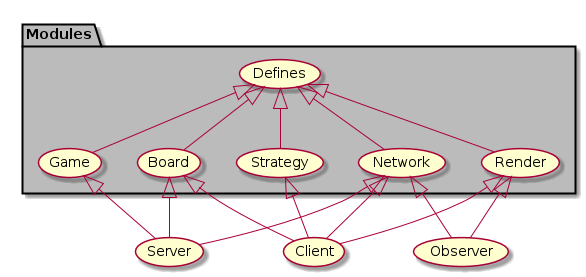
\includegraphics[scale=0.6]{diagramme.png}
\caption{Organisation en modules de notre projet}
\end{center}
\end{figure}


\sec{Synthèse}

Ce projet fut l'occasion pour nous de nous intéresser pour la première fois à l'implémentation des \textit{sockets} en C.

Il nous a également conduit à des questionnements de sécurité (vérification de règle) ou de stabilité (gestion des déconnexions).

\sec{Bibliographie}
Tutorial \textit{sockets} : \url{http://beej.us/guide/bgnet/output/html/singlepage/bgnet.html}


\end{document}
